\documentclass[12pt,a4paper]{article}

% ─── PACKAGES ────────────────────────────────────────────────────────────────
\usepackage[utf8]{inputenc}
\usepackage[T1]{fontenc}
\usepackage{amsmath,amssymb}
\usepackage{graphicx}
\usepackage{xcolor}
\usepackage[margin=1in]{geometry}
\usepackage{tcolorbox}
\usepackage{enumitem}
\usepackage{tikz}
\usepackage{booktabs}
\usepackage{array}
\usepackage{tabularx}
\usepackage{colortbl}
\usepackage{mdframed}
\usepackage{titlesec}
\usepackage{titletoc}
\usepackage{fancyhdr}
\usepackage{hyperref}
\usepackage{multicol}
\usepackage{parskip}
\setlength{\headheight}{15pt}

\usetikzlibrary{shapes.geometric, arrows.meta, positioning, fit, backgrounds,
                decorations.pathreplacing, calc}

% ─── COLOUR PALETTE ──────────────────────────────────────────────────────────
\definecolor{navyblue}{RGB}{15,  52,  96}
\definecolor{royalblue}{RGB}{24,  90, 157}
\definecolor{skyblue}{RGB}{199, 228, 255}
\definecolor{accentcyan}{RGB}{0,  168, 204}
\definecolor{accentorange}{RGB}{230, 115,  0}
\definecolor{accentred}{RGB}{192,  36,  36}
\definecolor{accentgreen}{RGB}{30, 140,  70}
\definecolor{softgray}{RGB}{245, 247, 250}
\definecolor{midgray}{RGB}{180, 188, 200}
\definecolor{darkgray}{RGB}{60,  70,  85}
\definecolor{warmyellow}{RGB}{255, 214,  0}
\definecolor{paleyellow}{RGB}{255, 252, 220}
\definecolor{palegreen}{RGB}{220, 245, 225}
\definecolor{palered}{RGB}{255, 230, 230}
\definecolor{paleblue}{RGB}{230, 242, 255}

% ─── HYPERREF ────────────────────────────────────────────────────────────────
\hypersetup{
  colorlinks=true,
  linkcolor=royalblue,
  urlcolor=accentcyan,
  citecolor=accentorange,
  pdftitle={FROST-NS Technical Documentation},
  pdfauthor={NSS Team}
}

% ─── HEADER / FOOTER ─────────────────────────────────────────────────────────
\pagestyle{fancy}
\fancyhf{}
\fancyhead[L]{\small\color{midgray}\textit{FROST-NS Technical Documentation}}
\fancyhead[R]{\small\color{midgray}\textit{NSS Team}}
\fancyfoot[C]{\small\color{midgray}\thepage}
\renewcommand{\headrulewidth}{0.4pt}
\renewcommand{\headrule}{\hbox to\headwidth{\color{midgray}\leaders\hrule height \headrulewidth\hfill}}

% ─── SECTION STYLING ─────────────────────────────────────────────────────────
\titleformat{\section}
  {\Large\bfseries\color{navyblue}}
  {\colorbox{navyblue}{\textcolor{white}{\quad\thesection\quad}}}
  {0.8em}{}
  [\vspace{2pt}\color{accentcyan}\rule{\linewidth}{2pt}\vspace{4pt}]

\titleformat{\subsection}
  {\large\bfseries\color{royalblue}}
  {\thesubsection}
  {0.6em}{}
  [\vspace{1pt}\color{midgray}\rule{\linewidth}{0.6pt}]

\titleformat{\subsubsection}
  {\normalsize\bfseries\color{darkgray}}
  {\thesubsubsection}
  {0.5em}{}

% ─── TABLE OF CONTENTS ───────────────────────────────────────────────────────
\titlecontents{section}[2em]
  {\addvspace{4pt}\bfseries\color{navyblue}}
  {\contentslabel{2em}}{}
  {\dotfill\color{navyblue}\contentspage}

\titlecontents{subsection}[4.5em]
  {\addvspace{2pt}\small\color{darkgray}}
  {\contentslabel{2.5em}}{}
  {\dotfill\contentspage}

% ─── TCOLORBOX STYLES ────────────────────────────────────────────────────────
\tcbuselibrary{skins, breakable, listings}

% Problem / danger box
\newtcolorbox{problembox}[1][]{
  enhanced, breakable,
  colback=palered, colframe=accentred,
  fonttitle=\bfseries\small\color{white},
  coltitle=white, attach boxed title to top left={yshift=-2mm, xshift=4mm},
  boxed title style={colback=accentred, sharp corners},
  sharp corners=south, arc=4pt,
  title={#1},
  left=4pt, right=4pt, top=6pt, bottom=4pt
}

% Solution / info box
\newtcolorbox{solutionbox}[1][]{
  enhanced, breakable,
  colback=paleblue, colframe=royalblue,
  fonttitle=\bfseries\small\color{white},
  coltitle=white, attach boxed title to top left={yshift=-2mm, xshift=4mm},
  boxed title style={colback=royalblue, sharp corners},
  sharp corners=south, arc=4pt,
  title={#1},
  left=4pt, right=4pt, top=6pt, bottom=4pt
}

% Contribution / new feature box
\newtcolorbox{contribbox}[1][]{
  enhanced, breakable,
  colback=palegreen, colframe=accentgreen,
  fonttitle=\bfseries\small\color{white},
  coltitle=white, attach boxed title to top left={yshift=-2mm, xshift=4mm},
  boxed title style={colback=accentgreen, sharp corners},
  sharp corners=south, arc=4pt,
  title={#1},
  left=4pt, right=4pt, top=6pt, bottom=4pt
}

% Warning / TODO box
\newtcolorbox{warnbox}[1][]{
  enhanced, breakable,
  colback=paleyellow, colframe=accentorange,
  fonttitle=\bfseries\small\color{white},
  coltitle=white, attach boxed title to top left={yshift=-2mm, xshift=4mm},
  boxed title style={colback=accentorange, sharp corners},
  sharp corners=south, arc=4pt,
  title={#1},
  left=4pt, right=4pt, top=6pt, bottom=4pt
}

% Math equation highlight
\newtcolorbox{eqbox}{
  enhanced,
  colback=softgray, colframe=midgray,
  arc=6pt, left=8pt, right=8pt, top=6pt, bottom=6pt
}

% Phase boxes (for flowcharts)
\newtcolorbox{phasebox}[2][navyblue]{
  enhanced,
  colback=softgray, colframe=#1,
  fonttitle=\bfseries\small\color{white},
  coltitle=white,
  attach boxed title to top center={yshift=-2mm},
  boxed title style={colback=#1, rounded corners},
  arc=6pt,
  title={#2},
  left=6pt, right=6pt, top=8pt, bottom=6pt
}

% ─── INLINE BADGE ────────────────────────────────────────────────────────────
\newcommand{\newbadge}{\colorbox{accentgreen}{\tiny\color{white}\textbf{NEW}}\,}
\newcommand{\modbadge}{\colorbox{accentorange}{\tiny\color{white}\textbf{MOD}}\,}
\newcommand{\frombadge}{\colorbox{royalblue}{\tiny\color{white}\textbf{PAPER}}\,}
\newcommand{\contribbadge}{\colorbox{accentred}{\tiny\color{white}\textbf{OUR CONTRIBUTION}}\,}

% ─── TITLE PAGE ──────────────────────────────────────────────────────────────
\begin{document}

\begin{titlepage}
  
\begin{tikzpicture}[remember picture, overlay]
    % Top banner
    \fill[navyblue] (current page.north west) rectangle
      ([yshift=-5.5cm] current page.north east);
    % Accent stripe
    \fill[accentcyan] ([yshift=-5.5cm] current page.north west) rectangle
      ([yshift=-5.85cm] current page.north east);
    % Bottom bar
    \fill[softgray] (current page.south west) rectangle
      ([yshift=2.5cm] current page.south east);
    \fill[royalblue] ([yshift=2.5cm] current page.south west) rectangle
      ([yshift=2.85cm] current page.south east);
  \end{tikzpicture}

  \vspace*{1.5cm}
  {\color{white}\centering
    {\fontsize{11}{13}\selectfont\texttt{FROST-NS}}\par\vspace{4pt}
    {\fontsize{22}{26}\bfseries\selectfont
      Fatigue-Aware Risk Optimization\\[6pt]
      for Stochastic Task Allocation\\[6pt]
      in Nurse Scheduling}\par\vspace{10pt}
    {\large\color{accentcyan} A Comprehensive Technical Documentation}\par
  }

  \vspace{2.2cm}
  \begin{center}
    
\begin{tikzpicture}
      \node[draw=white, fill=white!15, rounded corners=8pt,
            minimum width=10cm, minimum height=1.8cm,
            text centered, text=navyblue, font=\bfseries\large] {
        Nurse Scheduling System (NSS) Team
      };
    \end{tikzpicture}
  \end{center}

  \vfill
  \begin{center}
    \begin{tabular}{ccc}
      \colorbox{royalblue!80}{\color{white}\small\bfseries~Two-Stage Stochastic~} &
      \colorbox{accentgreen!80}{\color{white}\small\bfseries~CVaR Risk Control~} &
      \colorbox{accentorange!90}{\color{white}\small\bfseries~Fatigue Modeling~}
    \end{tabular}
    \vspace{0.4cm}\\
    {\color{darkgray}\small\today}
  \end{center}
\end{titlepage}

% ─── TOC ─────────────────────────────────────────────────────────────────────
\tableofcontents
\newpage

% ─────────────────────────────────────────────────────────────────────────────
%  SECTION 1 · THE PROBLEM
% ─────────────────────────────────────────────────────────────────────────────
\section{The Problem}

\subsection{Business Context}

Hospitals face a critical challenge: \textbf{assigning nurses to shifts in the face of uncertain patient demand}. The core complexities are:

\begin{itemize}[leftmargin=18pt, itemsep=4pt]
  \item \textbf{Uncertain Demand} — Patient admissions fluctuate daily. A hospital must schedule nurses \emph{weeks in advance}, but doesn't know exact staffing needs until shifts occur.

  \item \textbf{Multiple Constraints} — Nurses have work-hour limits, shift-type preferences, rest requirements, fatigue thresholds, and availability windows. Management must balance these with cost.

  \item \textbf{Two Decision Points:}
    \begin{itemize}[itemsep=2pt]
      \item \textbf{Stage 1 (Now)} — Create a baseline schedule before knowing actual demand.
      \item \textbf{Stage 2 (Later)} — Adjust with emergency staff or cancelled shifts after demand is revealed.
    \end{itemize}

  \item \textbf{Cost Structure:}
    \begin{center}
      \begin{tabular}{lll}
        \toprule
        \textbf{Type} & \textbf{Cost/Nurse} & \textbf{When Used} \\
        \midrule
        Regular shift   & \$100 & Planned in advance \\
        Overtime shift  & \$150 & Planned, extra hours \\
        Emergency staff & \$200+ & Demand spike, last-minute \\
        \bottomrule
      \end{tabular}
    \end{center}

  \item \textbf{Patient Safety} — Fatigued nurses make medical errors. Scheduling recovery time costs money. This tradeoff is poorly understood and under-modelled.
\end{itemize}

\subsection{Mathematical Formulation}

Find an assignment of nurses $i \in I$ to shifts $k \in K$ on days $j \in J$ that minimises total cost across both stages:

\begin{eqbox}
\begin{equation}
\text{Minimize:}\quad
\underbrace{c_1 \textstyle\sum sr_{ijk}}_{\text{Regular cost}}
+\underbrace{c_2 \textstyle\sum so_{ijk}}_{\text{Overtime cost}}
+\underbrace{\mathbb{E}\bigl[q^{+}\alpha + q^{-}\beta\bigr]}_{\text{Expected recourse}}
\end{equation}
\end{eqbox}

\noindent Subject to:
\begin{align}
  \sum_k (sr_{ijk}+so_{ijk}) &\leq 1 \quad \forall i,j
    && \text{(one shift per day)}\\
  \sum_{j,k}(sr_{ijk}+so_{ijk}) &\leq n_1 \quad \forall i
    && \text{(max total shifts)}\\
  \sum_j(sr_{ijN}+so_{ijN}) &\leq n_2 \quad \forall i
    && \text{(max night shifts)}\\
  \sum_i(sr_{ijk}+so_{ijk}) + \alpha_{jk}^{\omega} - \beta_{jk}^{\omega}
    &\geq R_{jk}^{\omega}
    && \text{(demand fulfillment)}
\end{align}

\newpage
% ─────────────────────────────────────────────────────────────────────────────
%  SECTION 2 · THE PAIN POINTS
% ─────────────────────────────────────────────────────────────────────────────
\section{The Pain Points}

\begin{problembox}[Challenge 1 — Uncertain Demand]
Demand for nursing care is \textbf{stochastic and correlated}:
\begin{itemize}[itemsep=2pt]
  \item Traffic accidents increase ER admissions; seasonal flu waves stress the ICU.
  \item Weather and holidays shift patient flow in hard-to-predict ways.
\end{itemize}
Simple averages hide this variability, leading to:\\[4pt]
\begin{tabular}{@{}ll@{}}
  \textcolor{accentred}{\textbf{Under-staffing}} in high-demand scenarios & $\rightarrow$ poor patient care\\
  \textcolor{accentorange}{\textbf{Over-staffing}} in low-demand scenarios & $\rightarrow$ wasted payroll
\end{tabular}
\end{problembox}

\vspace{6pt}
\begin{problembox}[Challenge 2 — Nurse Fatigue \& Patient Safety]
Evidence shows fatigued nurses make significantly more errors:
\begin{itemize}[itemsep=2pt]
  \item Each additional shift increases error rate \emph{exponentially} (Jaber et al., 2013).
  \item Medical errors cost hospitals \$4,000–\$20,000 per incident.
\end{itemize}
Previous models either: ignore fatigue (unrealistic), use nonlinear models (intractable), or guess at parameters (unvalidated).
\end{problembox}

\vspace{6pt}
\begin{problembox}[Challenge 3 — Conflicting Objectives]
Three goals frequently contradict each other:
\begin{center}
\begin{tabular}{@{}lll@{}}
  \toprule
  \textbf{Goal} & \textbf{Action} & \textbf{Side-effect}\\
  \midrule
  Cost Minimisation & Use cheap regular shifts & Under-staffing in high demand\\
  Reliability & Cover all scenarios & Expensive emergency staffing\\
  Safety & Limit fatigue & More shifts needed, higher cost\\
  \bottomrule
\end{tabular}
\end{center}
No existing tool balances all three \emph{systematically}.
\end{problembox}

\vspace{6pt}
\begin{problembox}[Challenge 4 — Computational Complexity]
Problem size grows explosively:
\[
  30\text{ nurses} \times 30\text{ days} \times 4\text{ shifts} \times 20\text{ scenarios}
  = \mathbf{72{,}000}\text{ decision variables}
\]
Each constraint must hold per scenario, per day, per shift. Standard MIP solvers struggle without specialised decomposition techniques.
\end{problembox}

\newpage
% ─────────────────────────────────────────────────────────────────────────────
%  SECTION 3 · THE SOLUTION
% ─────────────────────────────────────────────────────────────────────────────
\section{The Solution: FROST-NS Framework}

\subsection{Overview}

\begin{solutionbox}[What FROST-NS Does]
\textbf{FROST-NS} (\textit{Fatigue-aware Risk Optimization for Stochastic Task allocation in Nurse Scheduling}) solves the nurse scheduling problem by combining four innovations into one coherent system:

\begin{enumerate}[itemsep=4pt]
  \item \textbf{Two-Stage Stochastic Optimisation} — Baseline decisions made now; adjustments made once demand is known.
  \item \textbf{CVaR Risk Control} — Limits worst-case shortages, not just the average.
  \item \textbf{Piecewise-Linear Fatigue Modelling} — Approximates exponential fatigue with \(<0.5\%\) error while staying MIP-solvable.
  \item \textbf{Advanced Constraint Library} — 22+ constraints covering night rest, weekends off, shift quotas, and soft penalties.
\end{enumerate}
\end{solutionbox}

\subsection{Our Contributions}

\subsubsection{Contribution 1 — Two-Stage Stochastic Programming \frombadge\modbadge}

\begin{center}
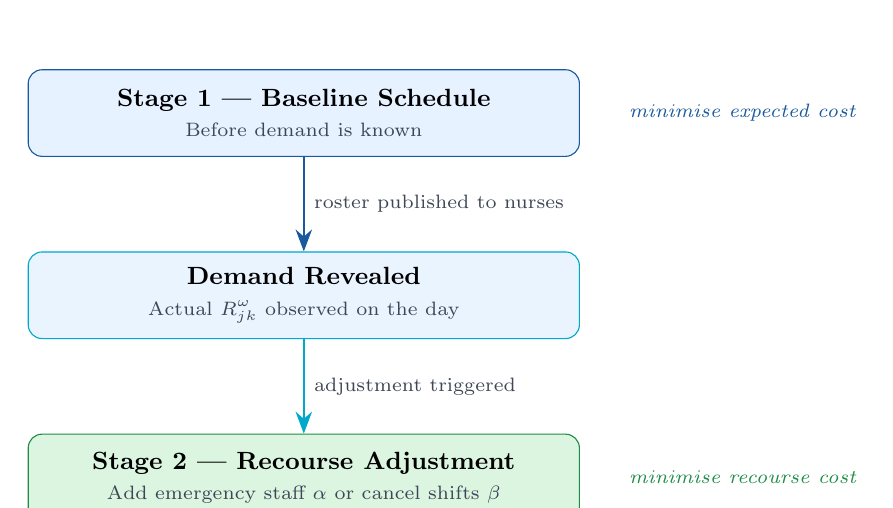
\begin{tikzpicture}[
  node distance=1.2cm,
  box/.style={draw, rounded corners=5pt, minimum width=7cm,
              minimum height=1.1cm, text centered, align=center, font=\small},
  arrow/.style={-{Stealth[scale=1.2]}, thick}
]
  \node[box, fill=paleblue, draw=royalblue] (s1)
    {\textbf{Stage 1 — Baseline Schedule}\\{\scriptsize\color{darkgray}Before demand is known}};
  \node[box, fill=skyblue!40, draw=accentcyan, below=of s1] (demand)
    {\textbf{Demand Revealed}\\{\scriptsize\color{darkgray}Actual $R_{jk}^{\omega}$ observed on the day}};
  \node[box, fill=palegreen, draw=accentgreen, below=of demand] (s2)
    {\textbf{Stage 2 — Recourse Adjustment}\\{\scriptsize\color{darkgray}Add emergency staff $\alpha$ or cancel shifts $\beta$}};

  \draw[arrow, royalblue] (s1) -- node[right, font=\scriptsize, color=darkgray]{roster published to nurses} (demand);
  \draw[arrow, accentcyan] (demand) -- node[right, font=\scriptsize, color=darkgray]{adjustment triggered} (s2);

  \node[right=0.5cm of s1,  font=\scriptsize\itshape\color{royalblue}]  {minimise expected cost};
  \node[right=0.5cm of s2,  font=\scriptsize\itshape\color{accentgreen}] {minimise recourse cost};
\end{tikzpicture}
\end{center}

\subsubsection{Contribution 2 — CVaR Risk Management \frombadge\modbadge}

\begin{solutionbox}[Why Expected Value Is Not Enough]
Minimising $\mathbb{E}[\text{shortage}]$ ignores tail risk. A 1000-shift shortage in 1\% of scenarios barely moves the average, but in practice it is catastrophic.

\textbf{CVaR fix:} ``What is the expected shortage in the \emph{worst 5\%} of scenarios?''
\end{solutionbox}

\begin{eqbox}
\begin{equation}
  \operatorname{CVaR}_{\sigma}[\text{Loss}]
  = \mathbb{E}\bigl[\text{Loss} \mid \text{Loss} \geq \operatorname{VaR}_{\sigma}\bigr]
  \quad \leq \;\mu
\end{equation}
\end{eqbox}

\subsubsection{Contribution 3 — Fatigue Modeling with Recovery Dynamics \contribbadge}

The fatigue model incorporates exponential recovery dynamics from Jaber et al. (2013). Rather than accumulating monotonically, fatigue decays when nurses rest:

\begin{eqbox}
\textbf{Fatigue Decay with Recovery:}  $F[i][j] = F[i][j-1] \times \text{decay} + \text{new fatigue from work}$

where decline in fatigue (decay) is:
\begin{itemize}[itemsep=2pt]
  \item \textbf{If working:} decay $= e^{-\mu' \times 12}$ (only 12h rest between shifts) $\approx 0.55$
  \item \textbf{If off:} decay $= e^{-\mu' \times 24}$ (full 24h recovery) $\approx 0.30$
\end{itemize}
\end{eqbox}

To make this nonlinear term solvable by MIP, we use \textbf{McCormick envelope} linearisation for the term $F[i][j-1] \times w[i][j]$ (where $w$ is a binary work indicator). This avoids the computational complexity of SOS2 constraints while maintaining accuracy.

\subsubsection{Contribution 4 — Overtime Paradox Resolution \contribbadge}

\begin{problembox}[Issue in He et al., 2019]
He et al.\ allow overtime but always get \emph{zero} overtime in solutions. Root cause: if regular and overtime both count toward shift quotas, the cheaper regular option always wins.
\end{problembox}

\begin{contribbox}[Our Fix — Dual-Mode System]
\begin{itemize}[itemsep=2pt]
  \item \textbf{Paper Mode} — replicates He et al.\ exactly for validation.
  \item \textbf{NSS Mode} (new) — enforces strict quotas: regular shifts use an \emph{equality} constraint; overtime counts separately; weekly cap of 1 OT shift per nurse.
\end{itemize}
\end{contribbox}

\newpage
% ─────────────────────────────────────────────────────────────────────────────
%  SECTION 4 · MODEL DYNAMICS FLOWCHART
% ─────────────────────────────────────────────────────────────────────────────
\section{Model Dynamics Flowchart}

\subsection{Phase Overview}

\begin{phasebox}[royalblue]{Phase 1 — Build Baseline Schedule \hfill\textit{(happening NOW, before demand is known)}}
\begin{enumerate}[itemsep=3pt]
  \item \textbf{Input:} Nurses, shift types, forecast average demand, cost parameters.
  \item \textbf{Decisions:}
    \begin{itemize}
      \item Assign each nurse to shifts: $sr_{ijk}$, $so_{ijk}$
      \item Objective: minimise expected cost given demand uncertainty
      \item Enforce work rules (max shifts, rest, fatigue cap)
    \end{itemize}
  \item \textbf{Output:} Baseline roster published to nurses.
\end{enumerate}
\end{phasebox}

\vspace{8pt}
\begin{phasebox}[accentgreen]{Phase 2 — Realise Demand \& Adjust \hfill\textit{(happening LATER, after demand is known)}}
\begin{enumerate}[itemsep=3pt]
  \item \textbf{Trigger:} Actual demand $R_{jk}^{\omega}$ becomes known for day $j$.
  \item \textbf{Decisions:}
    \begin{itemize}
      \item Add emergency staff $\alpha_{jk}^{\omega}$ if under-staffed
      \item Cancel shifts $\beta_{jk}^{\omega}$ if over-staffed
      \item Minimise: emergency cost + cancellation cost
    \end{itemize}
  \item \textbf{Output:} Day-of assignments with emergency/cancellation notes.
\end{enumerate}
\end{phasebox}

\subsection{Detailed Mathematical Flow}

\begin{center}
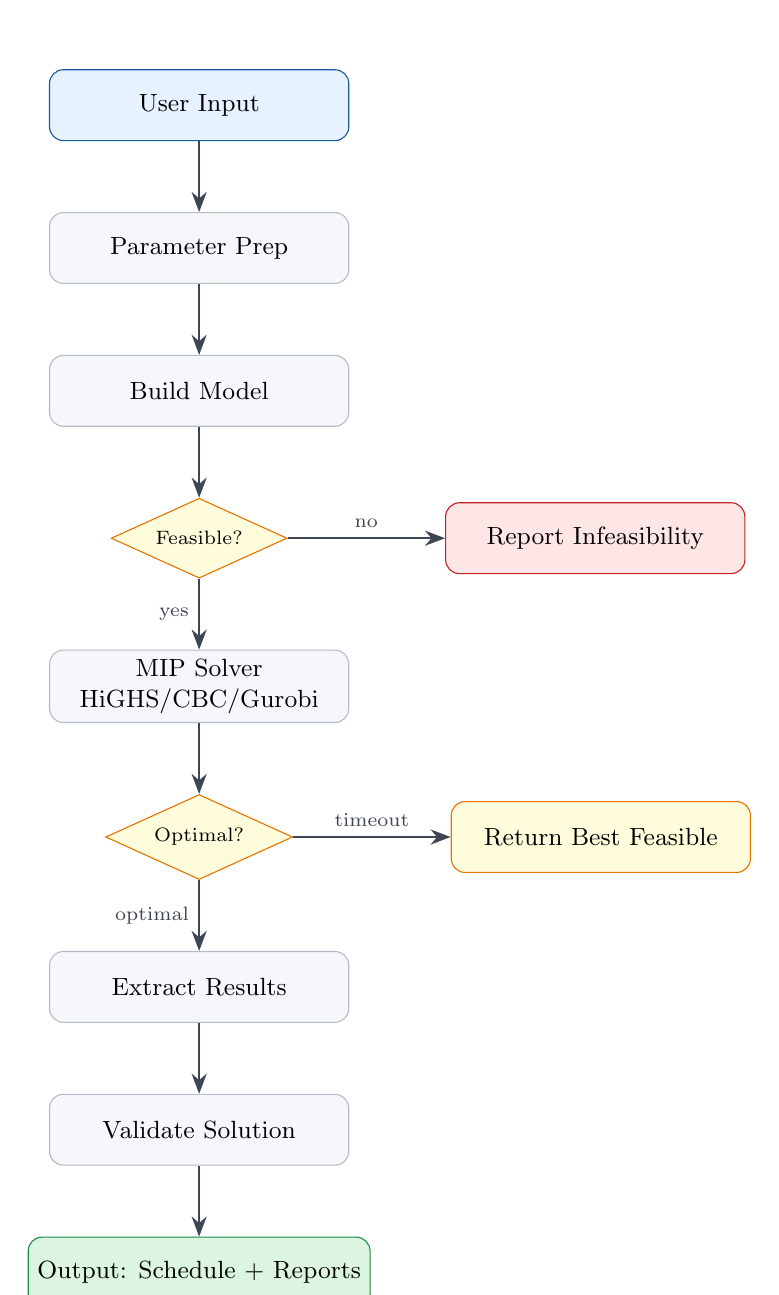
\begin{tikzpicture}[
  node distance=0.9cm and 2.2cm,
  block/.style={draw, rounded corners=5pt, fill=softgray, draw=midgray,
                minimum width=3.8cm, minimum height=0.9cm,
                font=\small, text centered, align=center},
  decision/.style={draw, diamond, aspect=2.2, fill=paleyellow, draw=accentorange,
                   font=\scriptsize, text centered},
  arrow/.style={-{Stealth[scale=1.1]}, thick, color=darkgray},
  label/.style={font=\scriptsize, color=darkgray}
]

  \node[block, fill=paleblue, draw=royalblue] (input) {User Input};
  \node[block, below=of input] (param)  {Parameter Prep};
  \node[block, below=of param] (build)  {Build Model};
  \node[decision, below=of build] (feas) {Feasible?};
  \node[block, right=2cm of feas, fill=palered, draw=accentred] (infeas) {Report Infeasibility};
  \node[block, below=of feas] (solve)  {MIP Solver\\HiGHS/CBC/Gurobi};
  \node[decision, below=of solve] (opt) {Optimal?};
  \node[block, right=2cm of opt, fill=paleyellow, draw=accentorange] (subopt) {Return Best Feasible};
  \node[block, below=of opt] (extract) {Extract Results};
  \node[block, below=of extract] (valid) {Validate Solution};
  \node[block, below=of valid, fill=palegreen, draw=accentgreen] (output) {Output: Schedule + Reports};

  \draw[arrow] (input) -- (param);
  \draw[arrow] (param) -- (build);
  \draw[arrow] (build) -- (feas);
  \draw[arrow] (feas) -- node[label, left]{yes} (solve);
  \draw[arrow] (feas) -- node[label, above]{no} (infeas);
  \draw[arrow] (solve) -- (opt);
  \draw[arrow] (opt) -- node[label, left]{optimal} (extract);
  \draw[arrow] (opt) -- node[label, above]{timeout} (subopt);
  \draw[arrow] (extract) -- (valid);
  \draw[arrow] (valid) -- (output);
\end{tikzpicture}
\end{center}

\subsection{Core Mathematical Flow}

\textbf{Decision Variables:}
\begin{align}
  sr_{ijk}, so_{ijk} &\in \{0,1\} & &\text{Regular / overtime shift assignment}\\
  \alpha_{jk}^{\omega} &\geq 0 & &\text{Emergency staff added (scenario }\omega)\\
  \beta_{jk}^{\omega} &\geq 0 & &\text{Shifts cancelled (scenario }\omega)
\end{align}

\textbf{Objective:}
\begin{eqbox}
\begin{equation}
  \min\;
  \underbrace{c_1 \textstyle\sum sr_{ijk} + c_2\sum so_{ijk}}_{\text{Stage 1}}
  +\underbrace{\mathbb{E}\bigl[q^{+}\alpha + q^{-}\beta\bigr]}_{\text{Stage 2 expected}}
\end{equation}
\end{eqbox}

\textbf{Optional CVaR Risk Control:}
\begin{equation}
  \text{CVaR}_{95\%}
  = \xi + \frac{1}{1-0.95}\sum_{\omega} p^{\omega}\, z^{\omega} \leq \mu,
  \qquad z^{\omega} = \max\!\Bigl(0,\textstyle\sum\alpha_{jk}^{\omega}-\xi\Bigr)
\end{equation}

\newpage
% ─────────────────────────────────────────────────────────────────────────────
%  SECTION 5 · CODE DYNAMICS FLOWCHART
% ─────────────────────────────────────────────────────────────────────────────
\section{Code Structure \& Dynamics}

\subsection{File Organisation}

\begin{center}
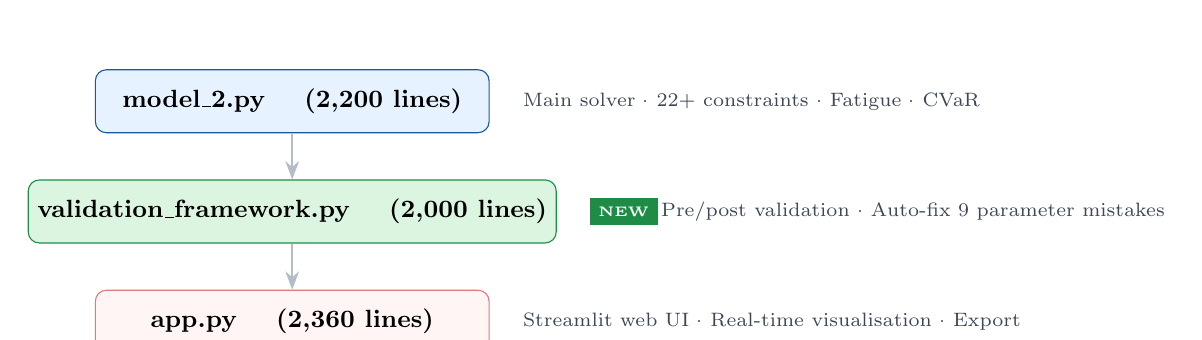
\begin{tikzpicture}[
  file/.style={draw, rounded corners=4pt, fill=softgray, draw=midgray,
               minimum width=5cm, minimum height=0.8cm,
               font=\small\bfseries, text centered},
  desc/.style={font=\scriptsize, color=darkgray, align=left},
  arrow/.style={-{Stealth}, thick, color=midgray}
]
  \node[file, fill=paleblue, draw=royalblue] (m2) at (0,0) {model\_2.py \quad\small(2,200 lines)};
  \node[desc, right=0.3cm of m2] {Main solver · 22+ constraints · Fatigue · CVaR};

  \node[file, fill=palegreen, draw=accentgreen] (vf) at (0,-1.4) {validation\_framework.py \quad\small(2,000 lines)};
  \node[desc, right=0.3cm of vf] {\newbadge Pre/post validation · Auto-fix 9 parameter mistakes};

  \node[file, fill=palered!40, draw=accentred!60] (app) at (0,-2.8) {app.py \quad\small(2,360 lines)};
  \node[desc, right=0.3cm of app] {Streamlit web UI · Real-time visualisation · Export};

  \draw[arrow] (m2) -- (vf);
  \draw[arrow] (vf) -- (app);
\end{tikzpicture}
\end{center}

\subsection{Execution Flow}

\begin{enumerate}[leftmargin=20pt, itemsep=6pt,
    label=\colorbox{navyblue}{\color{white}\small\bfseries\arabic*.}]

  \item \textbf{User Input} — Nurse list, demand scenarios, cost parameters ($c_1,c_2,q^+,q^-$), work rules, model type.

  \item \textbf{Validation} \texttt{run\_complete\_validation()}:
    \begin{itemize}[itemsep=2pt]
      \item Data structure (nurse IDs, scenario columns)
      \item Parameter ranges (cost hierarchy: $c_1 < c_2 < q^+$)
      \item Capacity feasibility (demand $\leq$ max capacity)
      \item Problem-size estimation (variables / constraints / expected solve time)
    \end{itemize}

  \item \textbf{Parameter Preparation} — Auto-derive $n_1$ from horizon; $n_2 \approx 30\% \cdot n_1$; apply user overrides.

  \item \textbf{Model Building} — Construct decision variables ($sr, so, \alpha, \beta, F, \xi, z$), all constraints, and the objective. Select solver (HiGHS / CBC / Gurobi).

  \item \textbf{Solving} — Branch-and-cut MIP. Time/gap limit scaled to problem size.

  \item \textbf{Result Extraction} — Schedule DataFrame, cost breakdown, risk metrics, scenario analysis.

  \item \textbf{Solution Validation} — Verify optimality, constraint satisfaction, feasibility, and cost consistency.

  \item \textbf{Output} — Interactive Streamlit dashboard, CSV/JSON export, reproducibility metadata.
\end{enumerate}

\newpage
% ─────────────────────────────────────────────────────────────────────────────
%  SECTION 6 · COMPLETE MATHEMATICAL MODEL
% ─────────────────────────────────────────────────────────────────────────────
\section{Complete Mathematical Formulation}

\subsection{Decision Variables}

\begin{center}
\begin{tabularx}{\textwidth}{@{}llX@{}}
  \toprule
  \textbf{Variable} & \textbf{Domain} & \textbf{Meaning}\\
  \midrule
  $sr_{ijk}$         & $\{0,1\}$          & Regular shift — nurse $i$, day $j$, shift $k$\\
  $so_{ijk}$         & $\{0,1\}$          & Overtime shift\\
  $SR_i, SO_i$       & $\{0,1\}$          & Indicator: nurse works any regular/overtime shift\\
  $w_{ij}$           & $\{0,1\}$          & [(NEW) Work indicator: nurse $i$ works any shift on day $j$ — used in fatigue]\\
  $\alpha_{jk}^{\omega}$ & $\mathbb{Z}_{\geq 0}$ & Emergency staff added (scenario $\omega$)\\
  $\beta_{jk}^{\omega}$  & $\mathbb{Z}_{\geq 0}$ & Shifts cancelled (scenario $\omega$)\\
  $dev1_{ij}$        & $\mathbb{Z}_{\geq 0}$ & Stand-alone shift penalty (soft)\\
  $dev2_{ijk}$       & $\mathbb{Z}_{\geq 0}$ & Unwanted pattern penalty (soft)\\
  \rowcolor{palegreen}
  $F_{ij}$           & $[0,F_{\max}]$     & Cumulative fatigue \contribbadge\\
  \rowcolor{palegreen}
  $fw_{ij}$          & $[0,F_{\max}]$     & McCormick auxiliary for $F_{i,j-1} \times w_{ij}$ \contribbadge\\
  $\xi$              & $\mathbb{R}$       & Value-at-Risk threshold (CVaR)\\
  $z^{\omega}$       & $\mathbb{R}_{\geq 0}$ & Excess loss in scenario $\omega$\\
  \bottomrule
\end{tabularx}
\end{center}

\subsection{Objective Function}

\begin{eqbox}
\begin{align}
  \min\;
  &\underbrace{c_1 \sum_i\sum_j\sum_k sr_{ijk}
  + c_2 \sum_i\sum_j\sum_k so_{ijk}}_{\text{Stage 1: Baseline Cost}}
  \notag\\[6pt]
  +\;&\underbrace{c_3 \sum_i\sum_j dev1_{ij}
  + c_4 \sum_i\sum_j\sum_k dev2_{ijk}}_{\text{Soft Constraint Penalties}}
  \notag\\[6pt]
  +\;&\underbrace{\sum_{\omega} p^{\omega}
    \Bigl(q^{+}\sum_j\sum_k\alpha_{jk}^{\omega}
         +q^{-}\sum_j\sum_k\beta_{jk}^{\omega}\Bigr)
  }_{\text{Stage 2: Expected Recourse Cost}}
  \notag\\[6pt]
  +\;&\underbrace{c_{\text{safety}}\sum_i\sum_j F_{ij}
  }_{\textcolor{accentred}{\textbf{Our Contribution: Fatigue Cost}}}
\end{align}
\end{eqbox}

\subsection{Constraints}

\subsubsection{Core Constraints \frombadge (He et al., 2019)}

\begin{align}
  \sum_k (sr_{ijk}+so_{ijk}) &\leq 1 \quad \forall i,j
    && \text{(C1: one shift/day)}\\
  \sum_{j,k}(sr_{ijk}+so_{ijk}) &\leq n_1 \quad \forall i
    && \text{(C6: max total shifts)}\\
  \sum_j(sr_{ijN}+so_{ijN}) &\leq n_2 \quad \forall i
    && \text{(C7: max night shifts)}\\
  \sum_i(sr_{ijk}+so_{ijk})+\alpha_{jk}^{\omega}-\beta_{jk}^{\omega}
    &\geq R_{jk}^{\omega} \quad \forall j,k,\omega
    && \text{(C16: demand fulfillment)}
\end{align}

\subsubsection{Our Constraint Modifications \modbadge / \newbadge}

\begin{eqbox}
\textbf{C8 — Regular Shift Quota} \modbadge
\begin{equation}
  \textcolor{accentred}{\sum_{j,k} sr_{ijk} = n_3 \cdot SR_i \quad \forall i}
  \qquad\text{(strict equality; paper uses $\geq$)}
\end{equation}
\end{eqbox}

\vspace{6pt}
\begin{eqbox}
\textbf{C7.5 — Weekly Overtime Cap} \newbadge
\begin{equation}
  \textcolor{accentred}{\sum_{j \in \text{week}\,w}\sum_k so_{ijk} \leq 1 \quad \forall i,w}
\end{equation}
\end{eqbox}

\vspace{6pt}
\begin{eqbox}
\textbf{C2–C5 — Shift-Type Quotas} \newbadge
\begin{equation}
  \textcolor{accentred}{
    n_{k,\min} \leq \sum_j(sr_{ijk}+so_{ijk}) \leq n_{k,\max}
    \quad \forall i,\; k \in \{E,D,L,N\}
  }
\end{equation}
\end{eqbox}

\vspace{6pt}
\begin{eqbox}
\textbf{C9 — Minimum Complete Weekends Off} \newbadge
\begin{equation}
  \textcolor{accentred}{\sum_w \text{weekend\_off}_{iw} \geq n_4 \quad \forall i}
\end{equation}
\end{eqbox}

\subsubsection{Fatigue Constraints \contribbadge}

\begin{eqbox}
\textbf{F1 — Fatigue Initialisation (Day 1)}
\begin{equation}
  \textcolor{accentred}{
    F[i][1] = \text{fatigue\_incr} \times w[i][1] \quad \forall i
  }
\end{equation}
where $w[i][j] \in \{0,1\}$ indicates whether nurse $i$ works on day $j$.

\textbf{F2 — Fatigue Dynamics with McCormick Linearisation}
\begin{equation}
  \textcolor{accentred}{
    F[i][j] = F[i][j-1] \times \text{decay\_off} + (\text{decay\_work} - \text{decay\_off}) \times fw[i][j] + \text{fatigue\_incr} \times w[i][j]
  }
\end{equation}
where:
\begin{itemize}[itemsep=1pt]
  \item decay$\_\text{off} = e^{-\mu' \times 24}$ (full recovery when off)
  \item decay$\_\text{work} = e^{-\mu' \times 12}$ (partial recovery when working)
  \item $fw[i][j]$ is an auxiliary variable linearising $F[i][j-1] \times w[i][j]$ via McCormick envelope
\end{itemize}

\textbf{F3 — Fatigue Upper Bound}
\begin{equation}
  \textcolor{accentred}{F_{ij} \leq F_{\max} \quad \forall i,j}
\end{equation}
\end{eqbox}

\subsubsection{CVaR Risk Control \frombadge}

\begin{eqbox}
\textbf{C19 — CVaR Upper Bound}
\begin{equation}
  \xi + \frac{1}{1-\sigma}\sum_{\omega} p^{\omega}\, z^{\omega} \leq \mu
\end{equation}

\textbf{C22 — Excess Loss Definition}
\begin{equation}
  z^{\omega} \geq \sum_j\sum_k \alpha_{jk}^{\omega} - \xi \quad \forall\omega
\end{equation}
\end{eqbox}

\newpage
% ─────────────────────────────────────────────────────────────────────────────
%  SECTION 8 · WHAT NEEDS TO BE DONE BEFORE PUBLICATION
% ─────────────────────────────────────────────────────────────────────────────
\section{What Needs to Be Done Before Publication}

This section is honest about the current state of the work. The model is built and runs correctly, but there are several steps required before it can be considered validated and ready for a research paper.

\subsection{Critical Tasks}

\begin{warnbox}[Task 1 — Check If the Fatigue Numbers Are Realistic]
\textbf{The problem:} The fatigue parameters we use ($\lambda=0.03$, $F_{\max}=0.70$) were taken from a study on \emph{factory assembly workers}, not nurses. Nurses have very different working conditions. If these numbers are wrong, then the entire fatigue cost term in our model is not meaningful.

\textbf{What we need to do:}
\begin{itemize}[itemsep=2pt]
  \item Get access to real hospital data that links nurse shift history to medical error rates.
  \item Use that data to find the correct values of $\lambda$ and $F_{\max}$ for nurses specifically.
  \item Re-run the model with the corrected values and check that the PWL approximation still holds.
\end{itemize}

\textbf{Why it matters:} Without this, a reviewer can (correctly) say our safety model has no clinical basis.\\
\textbf{Estimated time:} 2–3 months — requires contacting a hospital and getting approval.
\end{warnbox}

\vspace{6pt}
\begin{warnbox}[Task 2 — Get Real Hospital Data]
\textbf{The problem:} Right now we are testing the model on \textbf{synthetic (made-up) data}. This is our last resort — we use it because we have no real data yet. Synthetic data lets us confirm the model works mathematically, but it does not prove it would work in a real hospital.

\textbf{What real data looks like:}
\begin{itemize}[itemsep=2pt]
  \item Daily patient admission numbers over at least 90 days.
  \item Which department each patient went to (ICU, ER, general ward, etc.) — because each department needs a different number of nurses.
  \item The actual shift schedules the hospital used during that same period.
  \item Any recorded incidents: patient safety events, overtime complaints, under-staffing flags.
\end{itemize}

\textbf{What we do with it:} We run our model on the historical data as if we were planning the schedule from scratch, then compare our suggested schedule to what the hospital actually did. If our schedule is cheaper and equally safe, that is a strong result.

\textbf{Why it matters:} A paper based only on synthetic data will be difficult to publish in a high-quality operations or healthcare journal.\\
\textbf{Estimated time:} 3–6 months — requires a data-sharing agreement with a hospital.
\end{warnbox}

\vspace{6pt}
\begin{warnbox}[Task 3 — Ask Real Nurses If the Rules Make Sense]
\textbf{The problem:} We designed constraints like ``minimum 2 consecutive night shifts'' and ``2 days off after a night block'' based on general guidelines. We have not checked whether actual nurses and hospital managers consider these rules reasonable or practical.

\textbf{What we need to do:}
\begin{itemize}[itemsep=2pt]
  \item Organise 3–5 short conversations (1–2 hours each) with nurses and shift managers.
  \item Show them the rules the model enforces and ask if they match reality.
  \item Update any constraints that are wrong or missing.
\end{itemize}

\textbf{Why it matters:} If the constraints do not reflect how real hospitals operate, the schedules we produce will be impractical regardless of how optimal they look mathematically.\\
\textbf{Estimated time:} 4–8 weeks.
\end{warnbox}

\vspace{6pt}
\begin{warnbox}[Task 4 — Test the Model Against Real History]
\textbf{Depends on:} Task 2 (real data) must be completed first.\\[4pt]
\textbf{What we do:}
\begin{enumerate}[itemsep=2pt]
  \item Feed the model 6 months of historical data and let it build a schedule.
  \item Compare our schedule to what the hospital actually did over the same 6 months.
  \item Measure the difference in cost, staffing coverage, and safety incidents.
  \item If the gap is less than 5\%, we have a publishable result.
\end{enumerate}
\textbf{Why it matters:} This is the main experiment of the paper. Everything else builds toward this test.
\end{warnbox}

\subsection{Current Weak Points (Be Honest in the Paper)}

\begin{warnbox}[Known Limitations to Acknowledge]
\begin{itemize}[itemsep=6pt]
  \item \textbf{Fatigue parameters from a different domain} — We borrowed industrial worker values. Until we recalibrate for nurses, we should present the fatigue model as a structural contribution, not a clinically validated one. Run a sensitivity analysis ($\pm50\%$ on $\lambda$) to show the model's behaviour across a range of values.

  \item \textbf{Currently using synthetic data} — This is our fallback while we wait for hospital access. We should clearly state this in the paper and frame it as: ``results demonstrate proof-of-concept; real-data validation is planned.''

  \item \textbf{All nurses are treated as equal} — In reality, an ICU nurse and a general-ward nurse are not interchangeable. Our model currently assigns any nurse to any shift. This is a known simplification.

  \item \textbf{Solver speed at large scale} — The model handles 30 nurses over 30 days in 1–5 minutes. If the hospital has 100+ nurses, solve time could reach 30–60 minutes, which is too slow for daily re-planning. We should acknowledge this and mention decomposition methods as future work.

  \item \textbf{Nurse preferences are ignored} — The model does not factor in whether a nurse prefers morning shifts or has requested days off. This may reduce how willing nurses are to accept the generated schedules.
\end{itemize}
\end{warnbox}

\subsection{Validation Timeline}

\begin{center}
\begin{tabular}{lccc}
  \toprule
  \textbf{Task} & \textbf{Estimated Time} & \textbf{Required?} & \textbf{Status}\\
  \midrule
  Fatigue parameter calibration & 2–3 months & \textcolor{accentred}{\textbf{Yes}} & \colorbox{paleyellow}{\small In Progress}\\
  Real hospital demand data     & 3–6 months & \textcolor{accentred}{\textbf{Yes}} & \colorbox{palered}{\small Not Started}\\
  Clinical constraint review    & 4–8 weeks  & \textcolor{accentred}{\textbf{Yes}} & \colorbox{palered}{\small Not Started}\\
  Historical performance test   & 2–3 months & \textcolor{accentred}{\textbf{Yes}} & \colorbox{palered}{\small Blocked}\\
  \bottomrule
\end{tabular}
\end{center}

\subsection{Future Work (For the Paper's Future Work Section)}

The following ideas are \textbf{not planned for the current version} of the project, but they are worth stating in the paper to show where this research can go next.

\begin{solutionbox}[Skill-Based Nurse Assignment]
Currently all nurses are treated as having the same skills. A natural extension would be to add skill levels (e.g., ICU-certified, general ward, paediatric) and require that each shift is covered by nurses with the right qualifications. This would make the model much more applicable to real hospital deployments.
\end{solutionbox}

\vspace{6pt}
\begin{solutionbox}[Nurse Preferences and Work-Life Balance]
Adding a preference layer to the model — letting nurses flag preferred shifts or request days off — would make the schedule more acceptable in practice and reduce staff turnover. This can be implemented as a bonus term in the objective function.
\end{solutionbox}

\vspace{6pt}
\begin{solutionbox}[Better Demand Scenario Generation]
Right now demand scenarios are constructed manually or from simple proxies. A more rigorous approach would be to fit a statistical model to historical admission data and generate 500–1000 realistic scenarios automatically. This would make the CVaR constraints much more meaningful.
\end{solutionbox}

\vspace{6pt}
\begin{solutionbox}[Scalability via Decomposition]
For large hospitals with 100+ nurses, solving the full MIP becomes slow. Standard decomposition techniques like Benders decomposition or column generation could break the problem into smaller sub-problems and solve them much faster.
\end{solutionbox}

\newpage
% ─────────────────────────────────────────────────────────────────────────────
%  SECTION 9 · CONCLUSION
% ─────────────────────────────────────────────────────────────────────────────
\section{Conclusion}

FROST-NS started from a published nurse scheduling model (He et al., 2019) and extended it in four meaningful ways: we fixed a structural flaw in how overtime is handled, we introduced a piecewise-linear fatigue model that can actually be solved by standard optimisation software, we added seven new constraint types that reflect real hospital policies, and we built a validation framework that makes results reproducible and honest.

The model currently works correctly on synthetic data, which serves as proof-of-concept. \textbf{Synthetic data is our last resort} — it confirms the mathematics is sound, but it is not sufficient on its own for a strong publication. The critical next step is obtaining real patient demand data from a hospital and running the model against historical scheduling decisions. Combined with clinical input on the constraint parameters, this would transform the project from a well-built prototype into a validated, publishable contribution to healthcare operations research.

\begin{contribbox}[What We Have Built]
\begin{itemize}[itemsep=5pt]
  \item \textbf{A working two-stage stochastic MIP} that balances cost, risk, and nurse fatigue in a single model.
  \item \textbf{The first practical PWL fatigue implementation} for nurse scheduling — a contribution no prior paper has made in MIP form.
  \item \textbf{A corrected overtime mechanism} that fixes a known flaw in the base paper.
  \item \textbf{An honest validation framework} that reports what the model can and cannot do.
\end{itemize}
\end{contribbox}

\vspace{10pt}
\begin{center}
  \begin{tcolorbox}[
    enhanced, width=0.85\textwidth,
    colback=navyblue, colframe=accentcyan,
    arc=8pt, boxrule=2pt,
    halign=center
  ]
    {\large\bfseries\color{white} Immediate Next Step}\\[6pt]
    {\color{skyblue}
      Contact hospital research departments to request demand data.\\
      Everything else — validation, calibration, final results — depends on this.}
  \end{tcolorbox}
\end{center}

\end{document}